\chapter{微生物与感染}\label{ch:g9:microbes-and-infection}

从一年级“看不见的\omterm{def:g1:healthy-habits:germs}{病菌}”起，它们就一直
伴随着本书（\cref{def:g1:healthy-habits:germs}）：
它们在面包房里充当劳动力
（\cref{ch:g6:producing-our-food}），
在\omterm{def:g6:decomposers-and-soil:soil}{土壤}中充当\omterm{def:g6:decomposers-and-soil:decomposers}{分解者}，在医院病房里
成为不断进化的对手（\cref{ex:g9:how-species-change:resistance}）。
本章终于要为\omterm{def:g9:microbes-and-infection:sorted}{微生物}做一番完整的交代：
它们是什么，有害的少数如何发起攻击，
人体的外层防御——以及我们自己——如何守住门户。

\section{微生物世界}

\begin{definition}[微生物的分类]\label{def:g9:microbes-and-infection:sorted}
\emph{微生物}\index{微生物}——是
个体太小、肉眼无法直接看见的\omterm{def:g6:exploring-our-environment:components}{生物}。
主要分为以下几类：
\begin{itemize}
  \item \emph{细菌}\index{细菌}：\omterm{def:g6:cell-unit-of-life:unicellular}{单细胞}，
        没有真正的\omterm{def:g6:cell-unit-of-life:parts}{细胞核}，比你的\omterm{def:g5:first-look-at-cells:cell}{细胞}小得多，
        分裂迅速，
        是\cref{def:g6:cell-unit-of-life:unicellular}
        所说的\omterm{def:g6:cell-unit-of-life:unicellular}{单细胞}世界——无处不在，数量多得不可胜数；
  \item \emph{\omterm{def:g6:cell-unit-of-life:unicellular}{单细胞}\omterm{def:g6:decomposers-and-soil:decomposers}{真菌}及其他}：\omterm{ex:g6:producing-our-food:bread}{酵母}
        （\cref{ex:g6:producing-our-food:bread}）、霉菌的\omterm{def:g4:plants-without-seeds:spore}{孢子}、
        池塘水滴里的游动\omterm{def:g6:exploring-our-environment:components}{生物}；
  \item \emph{病毒}\index{病毒}：更小，性质也不同：
        它是一小段装在外壳里的\omterm{def:g9:heredity-and-traits:heredity}{遗传}信息
        （\cref{def:g9:genes-and-dna:dna}中的那些字母），
        外壳里\emph{没有\omterm{def:g5:first-look-at-cells:cell}{细胞}，也没有自己的生命}：
        病毒在进入活\omterm{def:g5:first-look-at-cells:cell}{细胞}之前什么也做不了；进入之后，
        它会让该\omterm{def:g5:first-look-at-cells:cell}{细胞}的读取机器转而
        复制入侵者的\omterm{def:g9:heredity-and-traits:heredity}{遗传}文本。
        按\cref{prop:g1:living-or-not:signs}所列的特征，
        病毒正处于生命的边缘。
\end{itemize}
\end{definition}

\begin{proposition}[大多无害，却常不可或缺]\label{prop:g9:microbes-and-infection:mostly}
\omterm{def:g9:microbes-and-infection:sorted}{微生物}“有害”的名声只是一种少数派的说法。
大多数\omterm{def:g9:microbes-and-infection:sorted}{微生物}对我们并无影响，许多还为我们服务：
\omterm{def:g6:decomposers-and-soil:decomposers}{分解者}（\cref{def:g6:decomposers-and-soil:decomposers}）、
食品生产中的“劳动力”、\omterm{def:g6:decomposers-and-soil:soil}{土壤}里的“化学家”，
以及你自身的\emph{常驻菌群}\index{常驻菌群}：
覆盖\omterm{def:g1:the-five-senses:sense}{皮肤}和肠道的数以万亿计的无害\omterm{def:g9:microbes-and-infection:sorted}{细菌}，帮助\omterm{def:g4:journey-of-food:digestion}{消化}，
并且仅凭占据地盘，就把入侵者挤出了立足之处。
只有少数\omterm{def:g9:microbes-and-infection:sorted}{微生物}——\emph{病原体}\index{病原体}——
才会引起疾病。
\end{proposition}
\admitted

\begin{example}[同一个身体，三种关系]\label{ex:g9:microbes-and-infection:relations}
此刻你的\omterm{def:g1:the-five-senses:sense}{皮肤}上：以十亿计的常驻菌，
守护着体表（关系一：互利）。
早餐的酸奶里：按要求变酸的“劳工”（关系二：受雇，
见\cref{ex:g6:producing-our-food:yogurt}）。
工具棚里一枚生锈的钉子上：破伤风杆菌的\omterm{def:g4:plants-without-seeds:spore}{孢子}，
正等待一道深伤口（关系三：\omterm{prop:g9:microbes-and-infection:mostly}{病原体}这一少数派，
也是
\cref{ch:g9:immune-defenses}的由来，
以及破伤风加强针的依据）。
\end{example}

\section{感染：分阶段的攻击}

\begin{definition}[感染的阶段]\label{def:g9:microbes-and-infection:stages}
\emph{感染}\index{感染}分为若干阶段，
每个阶段各有名称：
\begin{enumerate}
  \item \emph{传播}：\omterm{prop:g9:microbes-and-infection:mostly}{病原体}四处转移：
        接触过的物体表面和双手、咳嗽飞沫、
        受污染的食物和水、\omterm{prop:g4:journey-of-food:absorb}{血液}，
        以及\cref{def:g8:contraception:condom}所标示的
        性接触途径；
  \item \emph{侵入}：经由破口——\omterm{def:g1:the-five-senses:sense}{皮肤}割伤，或
        身体的开放门户：\omterm{def:g7:what-is-respiration:respiration}{呼吸}道、\omterm{def:g4:journey-of-food:tract}{消化道}，以及
        上述途径；
  \item \emph{增殖}：温暖、潮湿又有养料，入侵者开始分裂：
        \omterm{def:g9:microbes-and-infection:sorted}{细菌}在\cref{prop:g6:decomposers-and-soil:speed}所述
        \omterm{def:g6:exploring-our-environment:conditions}{条件}下，几小时内数量便翻倍；
        \omterm{def:g9:microbes-and-infection:sorted}{病毒}则把\omterm{def:g5:first-look-at-cells:cell}{细胞}变成
        复制作坊。
  \item \emph{疾病}：症状来自
        组织损伤本身、\omterm{def:g9:microbes-and-infection:sorted}{细菌}毒素，
        以及一部分（下一章）来自机体防御系统自身的战斗。
\end{enumerate}
\end{definition}

\begin{example}[两种入侵者的对比]\label{ex:g9:microbes-and-infection:contrast}
割伤处的\omterm{def:g9:microbes-and-infection:sorted}{细菌}对冬季的感冒\omterm{def:g9:microbes-and-infection:sorted}{病毒}。
\omterm{def:g9:microbes-and-infection:sorted}{细菌}：从破口侵入，在温暖潮湿的组织中
于\emph{\omterm{def:g5:first-look-at-cells:cell}{细胞}之间}繁殖，其废物毒害周围的\omterm{def:g6:exploring-our-environment:components}{环境}——
化脓手指的跳痛与脓液便是这样来的。
\omterm{def:g9:microbes-and-infection:sorted}{病毒}：附着在飞沫上，抵达气道内壁，
进入内壁的\omterm{def:g5:first-look-at-cells:cell}{细胞}本身，每个被劫持的\omterm{def:g5:first-look-at-cells:cell}{细胞}
在死亡前释放出大量拷贝——
其所经之处便是咽喉灼痛和流涕不止。
两者机制不同：能使前者“饿死”的抗生素，
对后者却无能为力，因为后者借用的是\emph{你的}
\omterm{def:g5:first-look-at-cells:cell}{细胞}机器，而针对它的药物很难精准作用。
\end{example}

\section{守住门户}

\begin{proposition}[最初的防线]\label{prop:g9:microbes-and-infection:doors}
在任何战斗开始之前，身体先守住边界：
\begin{itemize}
  \item \emph{\omterm{def:g1:the-five-senses:sense}{皮肤}}：干燥、分层、不断自我更新，这是一道
        屏障（\cref{def:g1:the-five-senses:sense}中的\omterm{def:g1:the-five-senses:sense}{感觉器官}，
        此时担负守卫之责）；
  \item \emph{黏膜及其“清扫工”}：\omterm{def:g7:what-is-respiration:respiration}{呼吸}道的
        清洁表面（\cref{prop:g7:lungs-and-gas-exchange:smoke}
        已表明其超负荷），泪液与\omterm{def:g4:journey-of-food:tract}{唾液}的冲洗化学作用，
        胃中的强酸浴
        （\cref{pb:g7:digestion-and-nutrients:1}
        在\omterm{def:g4:journey-of-food:digestion}{消化}食物的同时，
        将其杀菌）；
  \item \emph{\omterm{prop:g9:microbes-and-infection:mostly}{常驻菌群}}：常驻菌占据的
        地盘让入侵者难以落脚；
\end{itemize}
\omterm{def:g1:healthy-habits:hygiene}{卫生}措施也在加固这些屏障：
\cref{met:g1:healthy-habits:hands}中的肥皂洗手法
（现在能说清其完整机制——阻断传播）、安全饮水、
煮熟并冷藏保存的食物
（\cref{rem:g6:producing-our-food:goodbad}中
所说的不利\omterm{def:g6:exploring-our-environment:conditions}{条件}），消过毒的注射针头，以及\omterm{def:g8:contraception:condom}{避孕套}的屏障作用。
本书中的每一条\omterm{def:g1:healthy-habits:hygiene}{卫生}规则，
都是在阻断传播或侵入的某个阶段。
\end{proposition}
\admitted

\begin{omfigure}
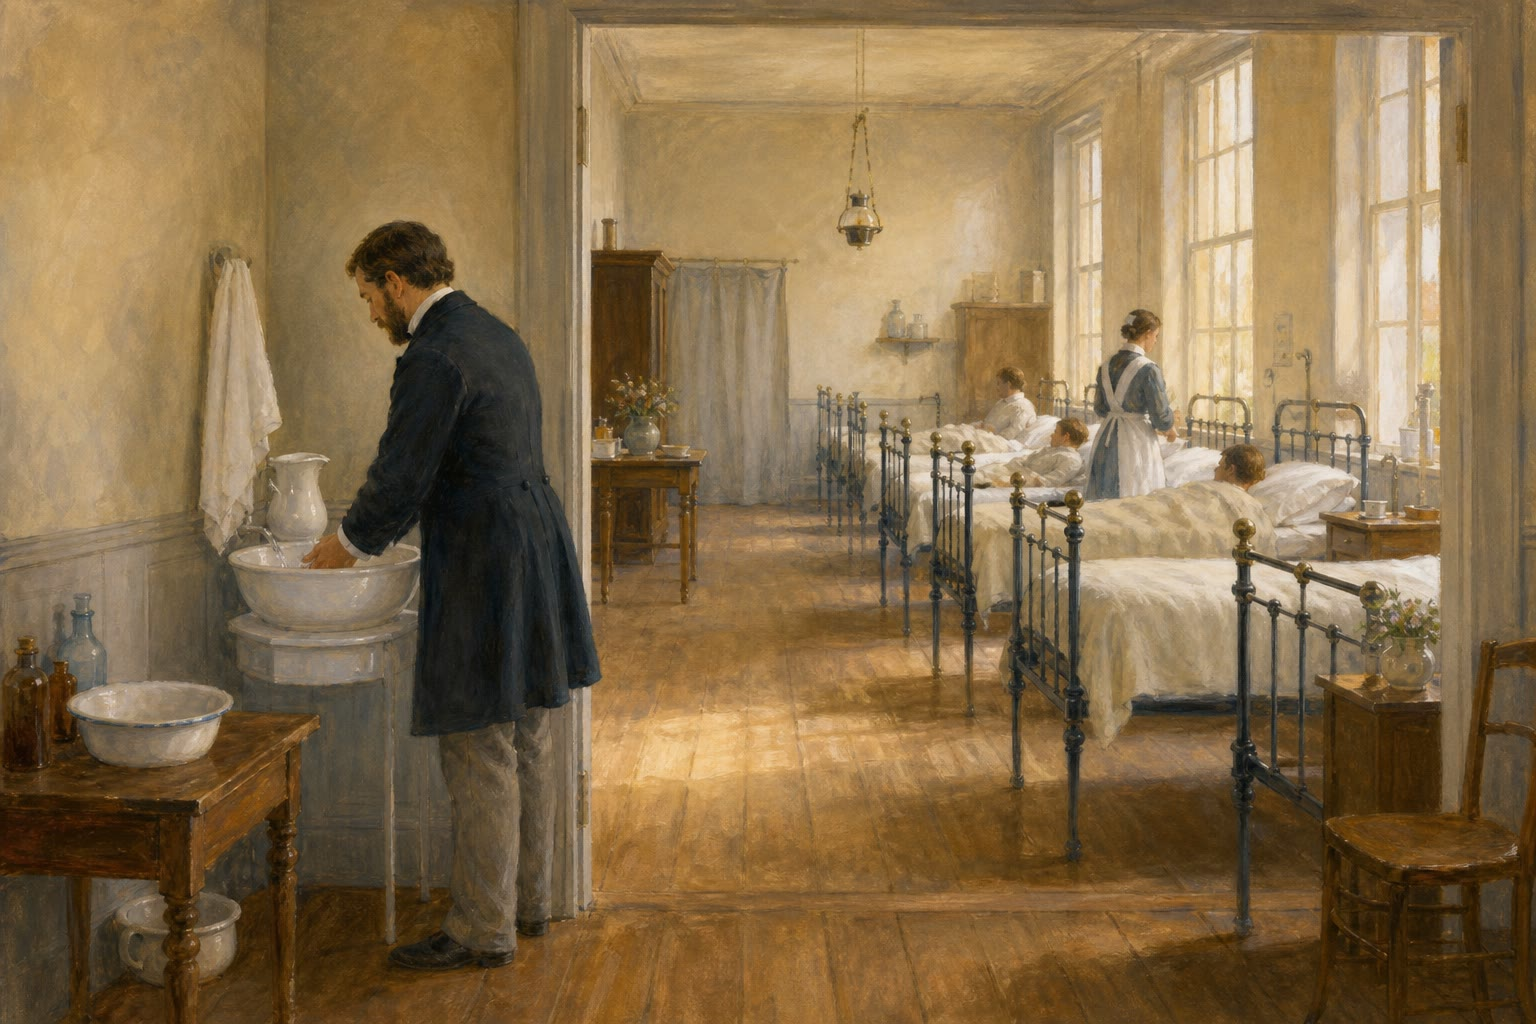
\includegraphics[width=0.6\linewidth]{images/book1/ai/g9-microbe-washing.jpg}

{\small 史上最便宜的药：
病房门口的一盆水，拦截了肉眼看不见的“信使”。}
\end{omfigure}

\begin{example}[两位让数字改变的医生]\label{ex:g9:microbes-and-infection:history}
两个人名撑起了这段历史。塞麦尔维斯，1840 年代的维也纳：
产褥热的死亡人数在他的产科病房里骤降，
原因是医生们在尸检室与接生之间洗手——
在人们看到“信使”之前，传播就已被切断。
巴斯德晚一代人出现，他揭示了“信使”本身：
不是“坏空气”，而是\omterm{def:g9:microbes-and-infection:sorted}{微生物}，
使葡萄酒变质、蚕死亡、伤口\omterm{def:g9:microbes-and-infection:stages}{感染}——
而加热（即他所称的\emph{巴氏消毒法}）或灭菌，
能将其制止。\omterm{def:g9:microbes-and-infection:sorted}{细菌}学说在一代人的时间里，
把医院从危险之地变成了防御之所。
\end{example}

\begin{omfigure}
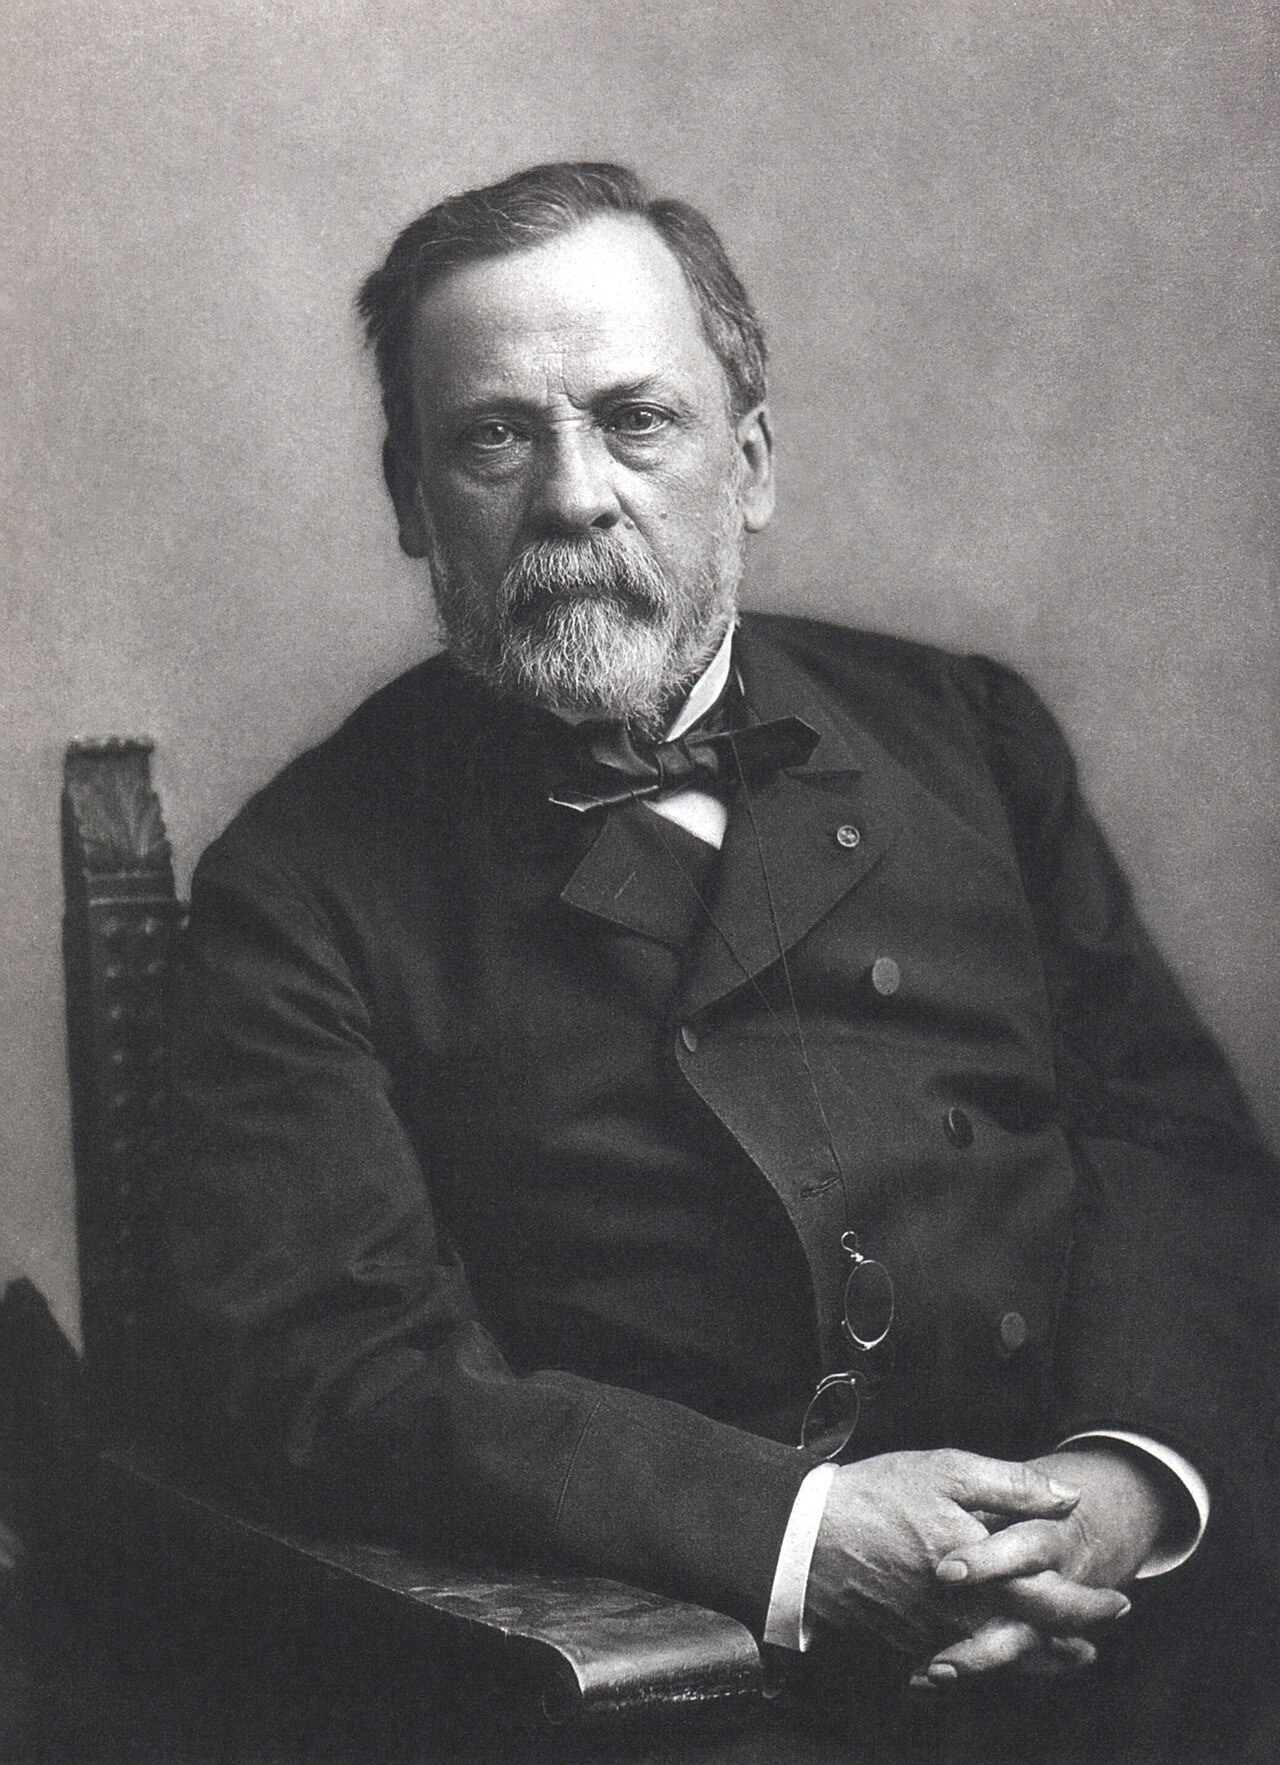
\includegraphics[width=0.42\linewidth]{images/book1/pasteur.jpg}

{\small 路易·巴斯德，保罗·纳达尔摄：
第一个揭示隐形“信使”本身的科学家。}
\end{omfigure}

\begin{method}[评估感染风险]\label{met:g9:microbes-and-infection:audit}
对任何情境——厨房、伤口、病房、人群：
\begin{enumerate}
  \item 指出可能的\omterm{prop:g9:microbes-and-infection:mostly}{病原体}及其类别
        （\omterm{def:g9:microbes-and-infection:sorted}{细菌}、\omterm{def:g9:microbes-and-infection:sorted}{病毒}、\omterm{def:g6:decomposers-and-soil:decomposers}{真菌}）；
  \item 追溯它到达你的传播途径；
  \item 找到它的侵入之门；
  \item 询问是什么使其增殖——\omterm{def:g6:exploring-our-environment:conditions}{温度}、\omterm{def:g6:exploring-our-environment:conditions}{湿度}、
        食物、时间；
  \item 阻断最便宜的环节：洗手、烹煮、覆盖、
        冷藏、灭菌、接种疫苗
        （\cref{ch:g9:immune-defenses}解释
        最后一项）。
\end{enumerate}
\end{method}

\section{练习}

\begin{exercise}[$\star$]\label{exo:g9:microbes-and-infection:1}
说出主要的\omterm{def:g9:microbes-and-infection:sorted}{微生物}类别，并说明\omterm{def:g9:microbes-and-infection:sorted}{病毒}的独特之处。
\end{exercise}

\begin{exercise}[$\star$]\label{exo:g9:microbes-and-infection:2}
什么是\omterm{prop:g9:microbes-and-infection:mostly}{常驻菌群}，它
发挥哪两种作用？
\end{exercise}

\begin{exercise}[$\star$]\label{exo:g9:microbes-and-infection:3}
列出\omterm{def:g9:microbes-and-infection:stages}{感染}的四个阶段，并各举一例。
\end{exercise}

\begin{exercise}[$\star$]\label{exo:g9:microbes-and-infection:4}
对比化脓伤口与感冒：
各种入侵者在何处增殖？
\end{exercise}

\begin{exercise}[$\star$]\label{exo:g9:microbes-and-infection:5}
说出四种第一道防线，以及各自所在的阶段。
\end{exercise}

\begin{exercise}[$\star$]\label{exo:g9:microbes-and-infection:6}
塞麦尔维斯的洗手措施阻断了什么，
巴斯德又增加了什么？
\end{exercise}

\begin{exercise}[$\star\star$]\label{exo:g9:microbes-and-infection:7}
为什么抗生素对感冒毫无作用？请
从两种入侵者的作用机制作答。
\end{exercise}

\begin{exercise}[$\star\star$]\label{exo:g9:microbes-and-infection:8}
以阶段阻断的方式，重新推导三条儿童\omterm{def:g1:healthy-habits:hygiene}{卫生}规则
（\cref{ch:g1:healthy-habits}），
并指出其机制。
\end{exercise}

\begin{exercise}[$\star\star$]\label{exo:g9:microbes-and-infection:9}
将\cref{met:g9:microbes-and-infection:audit}用于
夏日野餐的鸡肉沙拉，
在车内被晒热了三小时。
\end{exercise}

\begin{exercise}[$\star\star$]\label{exo:g9:microbes-and-infection:10}
为什么\emph{两项任务之间}洗手，
比频繁洗手更重要？（塞麦尔维斯的病房
给出了答案。）
\end{exercise}

\begin{exercise}[$\star\star$]\label{exo:g9:microbes-and-infection:11}
请把
\cref{ex:g9:how-species-change:resistance}中的病房
放到本章语境中来看：抗生素攻击的是哪一阶段，
其随意使用又会滋生什么？
\end{exercise}

\begin{exercise}[$\star\star\star$]\label{exo:g9:microbes-and-infection:12}
“\omterm{def:g9:microbes-and-infection:sorted}{病毒}是一段借用打印机的文字。”请展开这一比喻，
借助\cref{def:g9:genes-and-dna:dna}与
\cref{def:g9:microbes-and-infection:sorted}——并
以此说明\omterm{def:g9:microbes-and-infection:sorted}{病毒}为何处于生命的边缘，
以及为何难以用药物对付。
\end{exercise}

\section{问题：疫情笔记本}

\begin{problem}[{周末问题——一次校园疫情，
逐阶段追溯}]\label{pb:g9:microbes-and-infection:1}
某校（虚构）爆发疫情：一周之内，9B 班半数
学生报告发热与咳嗽；随后病例陆续出现在
其他班级。校医保存了一本疫情笔记，
请\omterm{def:g6:exploring-our-environment:components}{生物}课的同学帮忙读懂它。

\medskip\noindent\textbf{第一部分——追踪传播。}
\begin{enumerate}
  \item 首例病例——即索引病例——坐在 9B 班；其后
        八人与她同排，并同为她的乒乓球搭档。
        请指出最可能的传播途径，
        以及侵入的门户。
  \item 病例数起初每两天翻一番。此处体现的是
        哪一阶段的增殖规律，
        若\omterm{prop:g9:microbes-and-infection:mostly}{病原体}是\omterm{def:g9:microbes-and-infection:sorted}{病毒}，复制靠的是
        谁的机器？
  \item 校医的检查清单：发热的开始、咳嗽、
        咽喉灼痛。症状标志的是哪一阶段，
        它们又源于哪两个来源？
  \item 为何疫情恰好在本周两次
        全校集会时跨越了班级？
\end{enumerate}

\medskip\noindent\textbf{第二部分——反击行动。}
\begin{enumerate}[resume]
  \item 学校的措施：患病学生回家；
        开窗通风
        （见\cref{exo:g4:breathing:10}）；落实勤洗手；
        共用器材擦拭消毒。请为每项措施
        指出它阻断的阶段。
  \item 一位家长要求为全体学生使用抗生素。请拟写
        医生针对\omterm{def:g9:microbes-and-infection:sorted}{病毒}性疫情的答复，
        以及若抗生素仍被随意投放，
        则须提醒（见\cref{exo:g9:how-species-change:10}）
        所述的\omterm{prop:g9:how-species-change:selection}{自然选择}方面的警示。
  \item 食堂同时报告两例肠胃炎病例，
        均可追溯至一份未冷藏的甜点。请用
        \cref{met:g9:microbes-and-infection:audit}
        审计此支线疫情——
        \omterm{prop:g9:microbes-and-infection:mostly}{病原体}种类不同，所涉阶段亦不同。
  \item 校医为何要标出\emph{谁坐在哪里}，
        而不把病例当作随机分布？
        从传播角度看，疫情分布图是什么？
\end{enumerate}

\medskip\noindent\textbf{第三部分——复盘总结。}
\begin{enumerate}[resume]
  \item 按四个阶段，写出这次疫情的经过，
        从索引病例写到疫情消退。
  \item 疫情在尚未波及每一名学生前便已消退。
        请提出两种机制——一是措施的
        阻断作用，二是下一章的提示：
        部分学生已因去年的近缘毒株而获得免疫。
  \item 补写历史段落：学校的整体应对
        源自十九世纪的哪两项教训
        （见\cref{ex:g9:microbes-and-infection:history}）
        ？
  \item 以审计方法作为座右铭合上笔记本：
        用一句话说明，疫情在哪一环节
        阻断的成本最低。
\end{enumerate}
\end{problem}
